\documentclass[a4paper]{article}

\usepackage[T1]{fontenc}
\usepackage[utf8]{inputenc}
\usepackage[a4paper,margin=2cm]{geometry}
%\usepackage[francais]{babel}
%\usepackage{subfigure}
%\usepackage{fancyvrb}
%\usepackage{fancyhdr}
\usepackage{hyperref}
\usepackage{tabularx}
\usepackage{xcolor}
\usepackage{helvet}
%\usepackage{comment}
%\usepackage{lmodern}
\usepackage{varwidth}
\usepackage{tikz}
\usetikzlibrary{arrows,calc}
\usetikzlibrary{automata}
\usepackage{tikz-timing}
%\usetikzlibrary{matrix}
%\usetikzlibrary{shapes}
%\usetikzlibrary{positioning}
\usepackage{macros}
\usepackage{listings}
\usepackage{mathpazo}

% fontes tt avec gras (mots-clés)
\renewcommand{\ttdefault}{txtt}

\definecolor{deepgreen}{rgb}{0.09,0.32,0.09}
\definecolor{deepyellow}{rgb}{0.6,0.6,0}
\definecolor{kwcolor}{rgb}{0.6,0.1,0.1}

\lstset{
  language=Heptagon,% numbers=left, numberstyle=\small,
  basicstyle=\normalsize\ttfamily,captionpos=b,
  keywordstyle=\color{kwcolor},
  frame={tb}, rulesep=1pt, columns=fullflexible,
  xleftmargin=1cm, xrightmargin=1cm,
  mathescape=true
}



\tikzset{>=stealth'}

\tikzset{
  format/.style={rectangle,draw,color=blue,fill=blue!10},
  tool/.style={rectangle,draw,color=red,fill=red!10,rounded corners}
}

\title{Programming and controller synthesis with Heptagon/BZR and ReaX}

\author{Nicolas Berthier \and Gwenaël Delaval}

\date{}

\begin{document}

\maketitle

\section{Introduction}

Heptagon/BZR\footnote{\url{http://bzr.inria.fr}}\cite{delaval13:bzr_jdeds}
is a reactive language, belonging to the synchronous languages family,
whose main feature is to include discrete controller synthesis within
its compilation.

It is equipped with a behavioral contract mechanisms, where
assumptions can be described, as well as an ``enforce'' property part:
the semantics of this latter is that the property should be enforced
by controlling the behaviour of the node equipped with the
contract. This property will be enforced by an automatically built
controller, which will act on free controllable variables given by the
programmer.

ReaX\footnote{\url{http://reatk.gforge.inria.fr}}\cite{berthier14:_reax}
is a controller synthesis tool, dedicated to the control of
logico-numerical programs.

This report documents the integration of these two tools.

\section{Heptagon/BZR in a (small) nutshell}

Heptagon is a synchronous dataflow language, with a syntax allowing the
expression of control structures (e.g., switch or mode automata).

A typical Heptagon program will take as input a sequence of values,
and will output a sequence of values. Then, variables (inputs, outputs
or locals) as well as constants are actually variable or constant
\emph{streams}. The usual operators (e.g., arithmetic or Boolean
operators) are applied pointwise on these sequences of values.

Heptagon programs are structured in \emph{nodes}, which are provided
with \emph{inputs} and \emph{outputs}, and possibly local variables. A
node is defined by mean of a set of \emph{parallel equations},
defining the local variables and outputs' current values, as functions
of current inputs, other variables' values, and current state.

Figure~\ref{fig:hept-exple} shows a short Heptagon example. It
consists of a two-mode automaton, with a mode \emph{Up} in which the
output is increased by the current input value, and a mode \emph{Down}
in which the output is decreased.  The output \texttt{y}'s current
value is defined as the current value of the local variable
\texttt{x}, whose last value is recorded sp as tp be used in the
computation performed on the next step. In the \texttt{Up}
(resp. \texttt{Down}) mode, \texttt{x} is defined as the value of
\texttt{x} at the previous instant, increased (resp. decreased) by the
current value of the input \texttt{v}. The automaton stays in the
\texttt{Up} mode until \texttt{x} is greater or equal 10; meaning that
when this condition is true, the next mode will be the mode
\texttt{Down}.

\begin{figure}[hbp]
  \centering
\begin{lstlisting}
node twomodes(v:int) returns (y:int)
var last x : int = 0;
let
  y = x;
  automaton
    state Up
      do x = last x + v
      until x >= 10 then Down
    state Down
      do x = last x - v
      until x <= 0 then Up
  end
tel
\end{lstlisting}

  \scalebox{1.5}{

  \begin{tikztimingtable}
    v                    & 2D{2}  D{1} D{5}  D{2} D{1} D{0} D{3}\\
    State                & 4D{\texttt{Up}} 4D{\texttt{Down}}\\
    \texttt{twomodes}(v) & D{2} D{4} D{5} D{10} D{8} 2D{7} D{4}\\
  \end{tikztimingtable}
}
  \caption{Heptagon short example}
  \label{fig:hept-exple}
\end{figure}

The Heptagon/BZR language provides a \emph{contract} construct,
allowing the expression of assumptions on the environment (inputs)
(\texttt{assume} keyword), and guaranteed or enforced properties
(\texttt{enforce} keyword) on the outputs.

For example, the \texttt{twomodes} node given above can be enriched
with a contract, saying that if for every instant, $0 \leq \mathtt{v}
\leq 1$, then the property $0 \leq \mathtt{twomodes(v)} \leq 10$ will always hold (Fig.~\ref{fig:exple-contract}).

\begin{figure}[htbp]
  \centering
\begin{lstlisting}
node twomodes (v:int) = (y:int)

contract
  assume (v <= 1) & (v >= 0)
  enforce (o <= 10) & (o >= 0)

var last x : int = 0;
let
  y = x;
  automaton
    state Up
      do x = last x + v
      until x >= 10 then Down
    state Down
      do x = last x - v
      until x <= 0 then Up
  end
tel
\end{lstlisting}
  \caption{Example of contract in Heptagon/BZR}
  \label{fig:exple-contract}
\end{figure}

Contracts can also be provided with a declaration of
\emph{controllable variables}: these variables are local to the node,
and their value can be used into it. However, these variables are not
defined by the programmer. Their value will be given, during
execution, by a \emph{controller}, which will be computed offline by a
\emph{controller synthesis tool}.

Figure~\ref{fig:exple-contvar} shows how the \texttt{twomodes} node
can be equipped with a controllable variable \texttt{c}, which will
\emph{control} the transition between the two modes.

\begin{figure}[htbp]
  \centering
\begin{lstlisting}
node twomodes (v:int) = (y:int)

contract
  assume (v <= 1) & (v >= 0)
  enforce (o <= 10) & (o >= 0)
  with (c:bool)

var last x : int = 0;
let
  y = x;
  automaton
    state Up
      do x = last x + v
      until c then Down
    state Down
      do x = last x - v
      until c then Up
  end
tel
\end{lstlisting}
  \caption{Contract with one controllable variable}
  \label{fig:exple-contvar}
\end{figure}

We will see in the following sections how these contracts can be
handled by the ReaX verification and synthesis tool.

\section{Integration of Reax and Heptagon/BZR}

\subsection{Compilation chain}

Figure~\ref{fig:bzreax-compil} describes the full compilation process,
involving the Heptagon/BZR compiler (\texttt{heptc}) and the ReaX
controller synthesis tool.


\begin{figure}

\centering

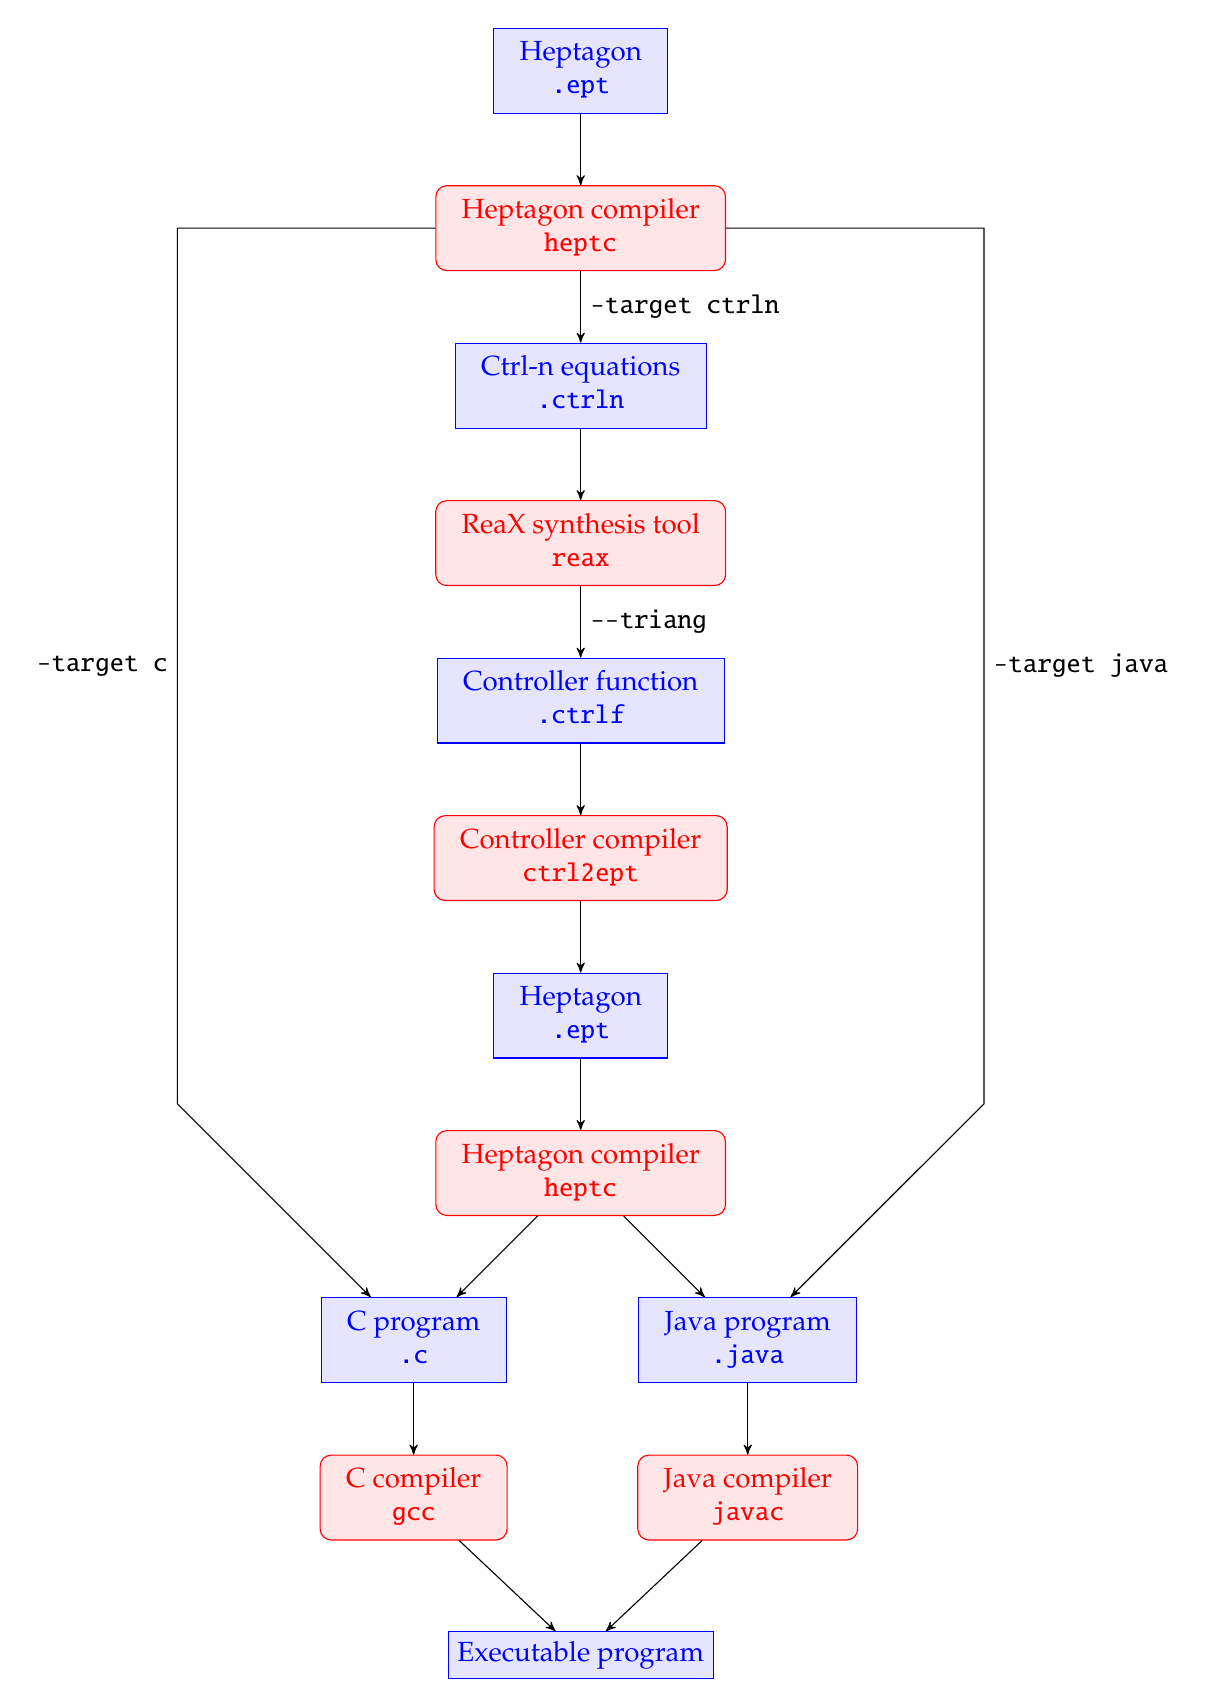
\begin{tikzpicture}[node distance=2cm]
  \node[format] (Heptagon) {\begin{tabular}{c}Heptagon\\\texttt{.ept}\end{tabular}};
  \node[tool,below of=Heptagon] (Heptc) {\begin{tabular}{c}Heptagon compiler\\\texttt{heptc}\end{tabular}};
  \node[format,below of=Heptc] (Ctrln) {\begin{tabular}{c}Ctrl-n equations\\\texttt{.ctrln}\end{tabular}};
  \node[tool,below of=Ctrln] (ReaX) {\begin{tabular}{c}ReaX synthesis tool\\\texttt{reax}\end{tabular}};
  \node[format,below of=ReaX] (Controller) {\begin{tabular}{c}Controller function\\\texttt{.ctrlf}\end{tabular}};
  \node[tool,below of=Controller] (Ctrl2ept) {\begin{tabular}{c}Controller compiler\\\texttt{ctrl2ept}\end{tabular}};
  \node[format,below of=Ctrl2ept] (HeptagonCtrlr) {\begin{tabular}{c}Heptagon\\\texttt{.ept}\end{tabular}};
  \node[tool,below of=HeptagonCtrlr] (HeptcCtrlr) {\begin{tabular}{c}Heptagon compiler\\\texttt{heptc}\end{tabular}};
  \node[format,below left of=HeptcCtrlr,node distance=3cm] (C) {\begin{tabular}{c}C program\\\texttt{.c}\end{tabular}};
  \node[format,below right of=HeptcCtrlr,node distance=3cm] (Java) {\begin{tabular}{c}Java program\\\texttt{.java}\end{tabular}};
  \node[tool,below of=C] (Gcc) {\begin{tabular}{c}C compiler\\\texttt{gcc}\end{tabular}};
  \node[tool,below of=Java] (Javac) {\begin{tabular}{c}Java compiler\\\texttt{javac}\end{tabular}};
  \coordinate (Middle) at ($(Gcc)!0.5!(Javac)$);
  \node[format,below of=Middle] (Exec) {Executable program};
  \draw[->] (Heptagon) -- (Heptc);
  \draw[->] (Heptc) -- node[right]{\texttt{-target ctrln}} (Ctrln);
  \draw[->] (Ctrln) -- (ReaX);
  \draw[->] (ReaX) -- node[right]{\texttt{--triang}} (Controller);
  \draw[->] (Controller) -- (Ctrl2ept);
  \draw[->] (Ctrl2ept) -- (HeptagonCtrlr);
  \draw[->] (HeptagonCtrlr) -- (HeptcCtrlr);
  \draw[->] (HeptcCtrlr) -- (C);
  \draw[->] (C) -- (Gcc);
  \draw[->] (Gcc) -- (Exec);
  \coordinate (A) at ($(C) + (-3,3)$);
  \draw[->] (Heptc) -| node[left,pos=0.75]{\texttt{-target c}} (A) --  (C);
  \coordinate (B) at ($(Java) + (3,3)$);
  \draw[->] (Heptc) -| node[right,pos=0.75]{\texttt{-target java}} (B) --  (Java);
  \draw[->] (HeptcCtrlr) -- (Java);
  \draw[->] (Java) -- (Javac);
  \draw[->] (Javac) -- (Exec);
\end{tikzpicture}

\caption{BZReaX full compilation chain}
\label{fig:bzreax-compil}
\end{figure}

The Heptagon compiler is usually used to generate target code in a
general-purpose language, like C (option \texttt{-target c}) or Java
(option \texttt{-target java}). This generated code is composed of two
functions for each Heptagon:
\begin{itemize}
\item a \emph{reset} function, used to reset the node's state ;
\item a \emph{step} function, which takes as input the current inputs
  of the node, update the current state, and computes the current
  outputs.
\end{itemize}

If a node is provided with a contract, then the ReaX
verification/synthesis tool can be used. The Heptagon backend towards
Ctrl-n equations (input format for ReaX) is activated with the
\texttt{-target ctrln} option.

The ReaX tool can then be used to synthesize (generate automatically)
a controller which, composed with the initial program, will give
values to the controllable variables so that the ``enforce'' property
stated by the contract is verified.

This controller is initially a Boolean predicate, over the values of
inputs, current state and controllable variable. The ReaX option
\texttt{-triang} allows the obtention of a function (in the same
Ctrl-n input format), giving values to the controllable variables,
functions of values of current inputs and state.

This controller function can then be translated into an Heptagon node
by the \texttt{ctrl2ept} tool. This Heptagon node is composed in
parallel with the initial one, by the technical mean of a node
instanciation. Thus, the generated code of this controller can be
compiled and linked with the code generated from the initial Heptagon
program.


\section{Verification of logico-numerical Heptagon programs with ReaX}

Heptagon/BZR contracts can be used, with the ReaX tool, to verify
logico-numerical programs.

Let us look back at the example given in
Figure~\ref{fig:exple-contract}, and name this program Modes (in a
file named \texttt{modes.ept}).
\begin{lstlisting}
node twomodes (v:int) = (y:int)

contract
  assume (v <= 1) & (v >= 0)
  enforce (o <= 10) & (o >= 0)

var last x : int = 0;
let
  y = x;
  automaton
    state Up
      do x = last x + v
      until x >= 10 then Down
    state Down
      do x = last x - v
      until x <= 0 then Up
  end
tel
\end{lstlisting}

We now want to check that the property stated by the contract is
guaranteed by the program. We begin then by compiling this program
towards the Ctrl-n input format :

\begin{alltt}
\textcolor{deepgreen}{> heptc -target ctrln modes.ept}
\end{alltt}

We obtain then a Ctrl-n program placed in a file named
\texttt{modes\_ctrln/twomodes.ctrln}. This file can be given as input
to the ReaX tool:
\begin{alltt}
\textcolor{deepgreen}{> reax -a 'sS:d=\{P:D\}' modes_ctrln/twomodes.ctrln}
[0.008 I Main] Reading node from `modes_ctrln/twomodes.ctrln'…
[0.024 I Supra] Variables(bool/num): state=(4/2), i=(0/1), u=(0/1), c=(0/0)
[0.024 I Df2cf] Preprocessing: discrete program
[0.024 I Verif] Forcing selection of power domain.
[0.024 I Synth] logico-numerical synthesis with powerset extension of power
                domain over strict convex polyhedra with BDDs:
[0.068 I sB] Building controller…
[0.072 I sB] Computing boundary transtions…
[0.072 I sB] Simplifying controller…
[0.072 I Synth] {\color{red}logico-numerical synthesis with powerset extension of power
                domain over strict convex polyhedra with BDDs succeeded.}
[0.072 I Main] Extracting generated controller…
[0.072 I Main] Checking generated controller…
[0.072 I Main] Outputting into `modes_ctrln/twomodes.ctrlr'…
\end{alltt}

The option \texttt{-a} followed by the string \verb+'sS:d={P:D}'+
defines the algorithme used for the verification. The algorithms
available are:
\begin{itemize}
\item \verb+'sB'+ for Boolean verification/synthesis (for Boolean
  programs, or whose Boolean abstraction is meaningful)
\item \verb+'sS'+ for verification/synthesis using abstract
  interpretation (over-approximation). The option \verb+'d={...}'+
  allows the selection of abstract domains :
  \begin{itemize}
  \item \texttt{I} selects the domain of \emph{intervals}, for
    programs with comparisons or operations between variables and
    constants ;
  \item \texttt{P} selects the domain of \emph{convex polyhedra},
    suitable for programs with comparisons or simple operations (sum or
    difference)
    between variables.
  \end{itemize}
  The second part (\texttt{\ldots:D}) of this string selects the
  \emph{powerset extension} of the power domain over the abstract
  domain, suitable for programs with mixed Boolean, modes and
  numerical operations on modes.
\end{itemize}

Our program involves operation between a state variable and an input
(\lstinline{last x + v}); thus we need to use the convex polyhedra
domain. Using a less precise domain such as intervals would lead to a
failed verification:
\begin{alltt}
\textcolor{deepgreen}{> reax -a 'sS:d={I:D}' modes_ctrln/twomodes.ctrln} 
[0.012 I Main] Reading node from `modes_ctrln/twomodes.ctrln'…
[0.024 I Supra] Variables(bool/num): state=(4/2), i=(0/1), u=(0/1), c=(0/0)
[0.024 I Df2cf] Preprocessing: discrete program
[0.024 I Verif] Forcing selection of power domain.
[0.025 I Synth] logico-numerical synthesis with powerset extension of power
                domain over intervals with BDDs:
[0.033 I Synth] {\color{red}logico-numerical synthesis with powerset extension of power
                domain over intervals with BDDs failed.}
\end{alltt}
              
\section{Controller synthesis on logico-numerical Heptagon programs with ReaX}

We add now a controllable variable to our \texttt{twomodes} node. This
controllable variable \texttt{c} will be used to control the
transition between the two modes:

\begin{lstlisting}
node twomodes (v:int) = (y:int)

contract
  assume (v <= 1) & (v >= 0)
  enforce (o <= 10) & (o >= 0)
  with (c:bool)

var last x : int = 0;
let
  y = x;
  automaton
    state Up
      do x = last x + v
      until not c then Down
    state Down
      do x = last x - v
      until not c then Up
  end
tel
\end{lstlisting}

The transition between \texttt{Up} and \texttt{Down} is no longer
defined as a condition on the current value of \texttt{x}, but
controlled by the controller, via the given value of \texttt{c}.

The full compilation of this program consists in:
\begin{enumerate}
\item Heptagon compilation towards C code and Ctrl-n equations; the
  \texttt{-s} option selects the simulated node (\texttt{twomodes})
\begin{alltt}
\textcolor{deepgreen}{> heptc -hepts -s twomodes -target c -target ctrln modes.ept}
\end{alltt}
\item Controller synthesis with ReaX (\texttt{--triang} option to
  obtain a function)
\begin{alltt}
\textcolor{deepgreen}{> reax -a 'sS:d=\{P:D\}' --triang modes_ctrln/twomodes.ctrln}
[0.008 I Main] Reading node from `modes_ctrln/twomodes.ctrln'…
[0.024 I Supra] Variables(bool/num): state=(4/2), i=(1/1), u=(0/1), c=(1/0)
[0.024 I Df2cf] Preprocessing: discrete program
[0.024 I Verif] Forcing selection of power domain.
[0.024 I Synth] logico-numerical synthesis with powerset extension of power
                domain over strict convex polyhedra with BDDs:
[0.072 I sB] Building controller…
[0.072 I sB] Computing boundary transtions…
[0.072 I sB] Simplifying controller…
[0.072 I Synth] logico-numerical synthesis with powerset extension of power
                domain over strict convex polyhedra with BDDs succeeded.
[0.092 I t.] Triangulation…ng…
[0.092 I Main] Extracting triangularized controller…
[0.092 I Main] Checking triangularized controller…
[0.092 I Main] Splitting triangularized controller…
[0.092 I Main] Extracting split triangularized controller…
[0.092 I Main] Checking split triangularized controller…
[0.092 I Main] Outputting into `modes_ctrln/twomodes.0.ctrls'…
\end{alltt}
\item Translation of the controller towards Heptagon
\begin{alltt}
\textcolor{deepgreen}{> ctrl2ept -n Modes.twomodes}
\end{alltt}
\item Compilation of the controller towards C
\begin{alltt}
\textcolor{deepgreen}{> heptc -target c modes_controller.ept}
\end{alltt}
\item Compilation and linking of all C files, obtaining an executable
  file for the simulation
\begin{alltt}
\textcolor{deepgreen}{> gcc -o sim -I/usr/local/lib/heptagon/c -Imodes_c -Imodes_controller_c
             modes_c/_main.c modes_c/modes.c modes_c/modes_types.c
             modes_controller_c/modes_controller.c
             modes_controller_c/modes_controller_types.c}
\end{alltt}
\end{enumerate}

The program can then be simulated:\\

\begin{tikztimingtable}
v &  2D{0} 4D{1} 2D{0} 8D{1} 3D{0} 10D{1} \\
twomodes(v) &  2D{0}D{1}D{2}D{3} 3D{4}D{5}D{6}D{7}D{8}D{9}D{10}D{9} 4D{8}D{7}D{6}D{5}D{4}D{3}D{2}D{1}D{0}D{1}D{2} \\
\end{tikztimingtable}

\section{Encapsulation: the BZReaX script}

The full compilation chain described in the previous section has been
encapsulated into a script named \texttt{bzreax}, whose scope is
described in Figure~\ref{fig:bzreax}.


\begin{figure}

\centering

\pgfdeclarelayer{background}
\pgfsetlayers{background,main}

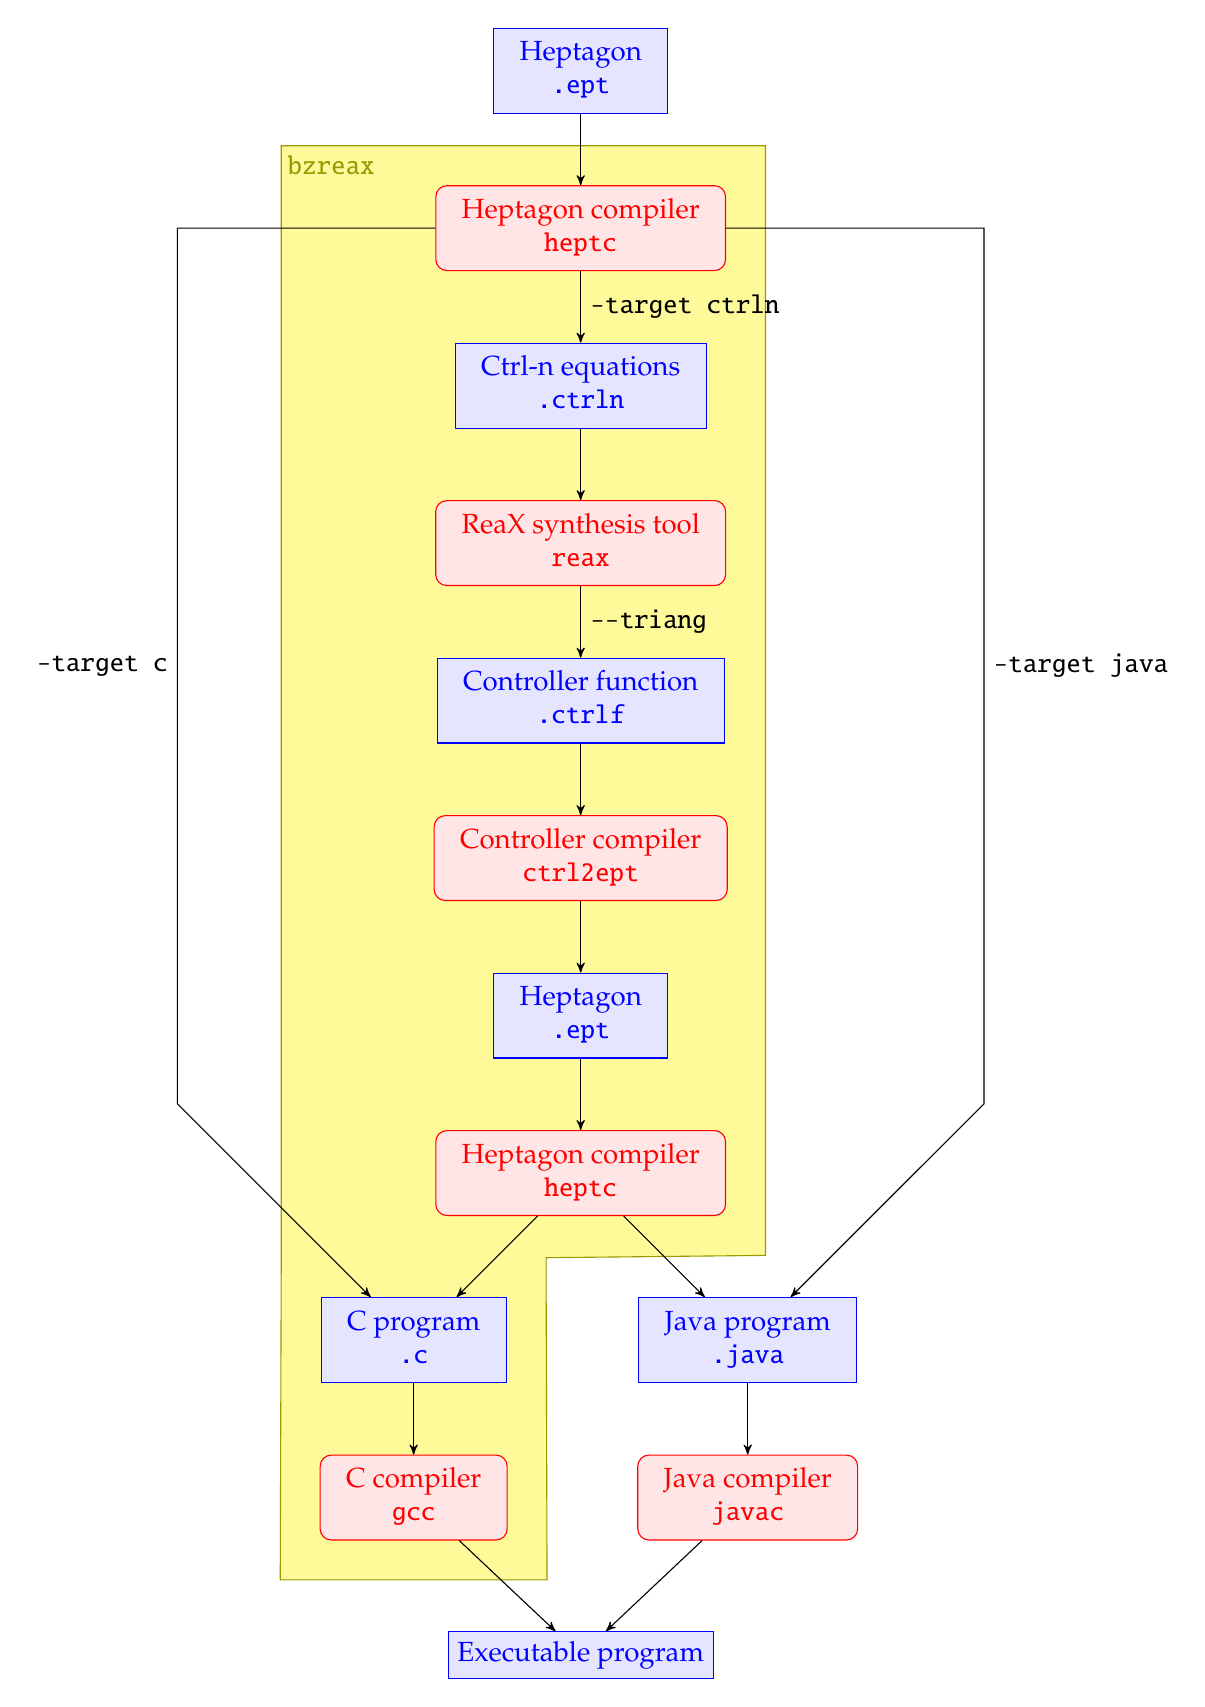
\begin{tikzpicture}[node distance=2cm]
  \node[format] (Heptagon) {\begin{tabular}{c}Heptagon\\\texttt{.ept}\end{tabular}};
  \node[tool,below of=Heptagon] (Heptc) {\begin{tabular}{c}Heptagon compiler\\\texttt{heptc}\end{tabular}};
  \node[format,below of=Heptc] (Ctrln) {\begin{tabular}{c}Ctrl-n equations\\\texttt{.ctrln}\end{tabular}};
  \node[tool,below of=Ctrln] (ReaX) {\begin{tabular}{c}ReaX synthesis tool\\\texttt{reax}\end{tabular}};
  \node[format,below of=ReaX] (Controller) {\begin{tabular}{c}Controller function\\\texttt{.ctrlf}\end{tabular}};
  \node[tool,below of=Controller] (Ctrl2ept) {\begin{tabular}{c}Controller compiler\\\texttt{ctrl2ept}\end{tabular}};
  \node[format,below of=Ctrl2ept] (HeptagonCtrlr) {\begin{tabular}{c}Heptagon\\\texttt{.ept}\end{tabular}};
  \node[tool,below of=HeptagonCtrlr] (HeptcCtrlr) {\begin{tabular}{c}Heptagon compiler\\\texttt{heptc}\end{tabular}};
  \node[format,below left of=HeptcCtrlr,node distance=3cm] (C) {\begin{tabular}{c}C program\\\texttt{.c}\end{tabular}};
  \node[format,below right of=HeptcCtrlr,node distance=3cm] (Java) {\begin{tabular}{c}Java program\\\texttt{.java}\end{tabular}};
  \node[tool,below of=C] (Gcc) {\begin{tabular}{c}C compiler\\\texttt{gcc}\end{tabular}};
  \node[tool,below of=Java] (Javac) {\begin{tabular}{c}Java compiler\\\texttt{javac}\end{tabular}};
  \coordinate (Middle) at ($(Gcc)!0.5!(Javac)$);
  \node[format,below of=Middle] (Exec) {Executable program};
  \draw[->] (Heptagon) -- (Heptc);
  \draw[->] (Heptc) -- node[right]{\texttt{-target ctrln}} (Ctrln);
  \draw[->] (Ctrln) -- (ReaX);
  \draw[->] (ReaX) -- node[right]{\texttt{--triang}} (Controller);
  \draw[->] (Controller) -- (Ctrl2ept);
  \draw[->] (Ctrl2ept) -- (HeptagonCtrlr);
  \draw[->] (HeptagonCtrlr) -- (HeptcCtrlr);
  \draw[->] (HeptcCtrlr) -- (C);
  \draw[->] (C) -- (Gcc);
  \draw[->] (Gcc) -- (Exec);
  \coordinate (A) at ($(C) + (-3,3)$);
  \draw[->] (Heptc) -| node[left,pos=0.75]{\texttt{-target c}} (A) --  (C);
  \coordinate (B) at ($(Java) + (3,3)$);
  \draw[->] (Heptc) -| node[right,pos=0.75]{\texttt{-target java}} (B) --  (Java);
  \draw[->] (HeptcCtrlr) -- (Java);
  \draw[->] (Java) -- (Javac);
  \draw[->] (Javac) -- (Exec);
  \begin{pgfonlayer}{background}
    \path[fill=yellow!40,draw=deepyellow] 
       ($(Heptc.north west) + (-0.5,0.5)$)
    -- ($(Heptc.north east) + (0.5,0.5)$)
    -- ($(HeptcCtrlr.south east) + (0.5,-0.5)$)
    -- ($(C.north east) + (0.5,0.5)$)
    -- ($(Gcc.south east) + (0.5,-0.5)$)
    -- ($(Gcc.south west) + (-0.5,-0.5)$)
    -- ($(C.north west) + (-0.5,0.5)$)
    |- cycle;
  \end{pgfonlayer}
  \node[anchor=north west,color=deepyellow] at ($(Heptc.north west) + (-2,0.5)$) {\texttt{bzreax}};
\end{tikzpicture}

\caption{BZReaX script}
\label{fig:bzreax}
\end{figure}

Thus, the full compilation of the program described in pthe previous
section can be obtained by:

\begin{alltt}
\textcolor{deepgreen}{> bzreax modes.ept twomodes -a 'sS:d=\{P:D\}' -s}
[0.008 I Main] Reading node from `modes_ctrln/twomodes.ctrln'…
[0.020 I Supra] Variables(bool/num): state=(4/2), i=(1/1), u=(0/1), c=(1/0)
[0.020 I Df2cf] Preprocessing: discrete program
[0.020 I Verif] Forcing selection of power domain.
[0.020 I Synth] logico-numerical synthesis with powerset extension of power
                domain over strict convex polyhedra with BDDs:
[0.056 I sB] Building controller…
[0.060 I sB] Computing boundary transtions…
[0.060 I sB] Simplifying controller…
[0.060 I Synth] logico-numerical synthesis with powerset extension of power
                domain over strict convex polyhedra with BDDs succeeded.
[0.072 I t.] Triangulation…ng…
[0.072 I Main] Extracting triangularized controller…
[0.072 I Main] Checking triangularized controller…
[0.072 I Main] Splitting triangularized controller…
[0.072 I Main] Extracting split triangularized controller…
[0.072 I Main] Checking split triangularized controller…
[0.072 I Main] Outputting into `modes_ctrln/twomodes.0.ctrls'…
Info: Loading module of controllers for node Modes.twomodes…
Info: Reading function from `modes_ctrln/twomodes.0.ctrls'…
Info: Outputting into `modes_controller.ept'…
Info: To launch the simulator, run: `hepts -mod Modes -node twomodes -exec ./sim'
\end{alltt}

\bibliographystyle{plain}
\bibliography{manual}


\end{document}
